\documentclass[11pt]{article}
\usepackage[utf8]{inputenc}
\usepackage[T1]{fontenc}
\usepackage{amsmath}
\usepackage{amsfonts}
\usepackage{amssymb}
\usepackage[version=4]{mhchem}
\usepackage{stmaryrd}
\usepackage{hyperref}
\hypersetup{colorlinks=true, linkcolor=blue, filecolor=magenta, urlcolor=cyan,}
\urlstyle{same}
\usepackage{multirow}
\usepackage{graphicx}
\usepackage[export]{adjustbox}
\graphicspath{ {./images/} }

\begin{document}
Benefits of Managed Futures Funds

A more direct way to examine the attractiveness of a managed futures investment is to analyze the performance of managed futures traders.

\section*{Research Regarding the Benefits of Managed Futures Funds}
In 1983, John Lintner presented one of the first academic papers on the topic of managed futures funds and their benefits. His analysis was designed to examine the risk-return characteristics of managed futures accounts or funds. ${ }^{1}$ Lintner, J. (1996), The Potential Role of Managed Commodity-Financial Futures Accounts (and/or Funds) in Portfolios of Stocks and Bonds, in The Handbook of Managed Futures: Performance, Evaluation and Analysis, edited by Carl Peters and Ben Warwick (New York: McGraw-Hill Professional), pp. 99-137, originally presented to the Analysts Federation in 1983. In this study, Lintner concluded that "the combined portfolios of stocks (or stocks and bonds) after including judicious investments ... in managed futures accounts (or funds) show substantially less risk at every possible level of expected return than portfolios of stocks (or stocks and bonds) alone."

Lintner's work provided an initial academic basis for investing in managed futures. Other early studies that followed his research both challenged and supported his results. A series of studies by Elton, Gruber, and Rentzler in 1987, 1989, and 1990, known as the EGR studies, examined public commodity pools and, unlike Lintner, found little evidence of the benefits of managed futures. ${ }^{2}$ Edwin J. Elton, Martin J. Gruber, and Joel C. Rentzler (1987), Professionally Managed, Publicly Traded Commodity Funds, Journal of Business 60 (no. 2): 175-99; New Public Offerings, Information, and Investor Rationality: The Case of Publicly Offered Commodity Funds, Journal of Business 62 (1989): 1-15; The Performance of Publicly Offered Commodity Funds, Financial Analysts Journal 46 (1987): 23-30. However, other analyses of managed futures supported their inclusion in investment portfolios. Some of these later analyses attempted to address data issues in the EGR studies. The EGR studies looked at public commodity pools, known to have been a very expensive way to invest in managed futures. Later analyses directly examined the returns of managed futures traders and found evidence that, on average, managed futures provide attractive risk-adjusted returns, especially if the performance is measured in the context of a diversified portfolio of stocks and bonds.

Unlike previous studies that examined the benefits of CTAs either as a standalone investment or in the context of portfolios consisting of traditional asset classes, Kat (2002) examined the possible role of managed futures in portfolios of stocks, bonds, and hedge funds. ${ }^{3}$ Harry M. Kat (November 1, 2002), Managed Futures and Hedge Funds: A Match Made in Heaven, Research paper, Cass Business School, London. He found that allocating to managed futures allows investors to achieve a very substantial degree of overall risk reduction at limited costs in terms of lower returns or skewness. Apart from their lower expected returns, managed futures appear to be more effective diversifiers than hedge funds. The paper concluded that adding managed futures to a portfolio of stocks and bonds will reduce that portfolio's standard deviation more and quicker than hedge funds will, and without the undesirable side effects in terms of lower skewness and higher kurtosis. Finally, Kat observed that overall portfolio standard deviation can be further reduced by combining both hedge funds and managed futures with stocks and bonds. Again, it is worth repeating that these results are, to some degree, time dependent and can change dramatically over short periods of time.

Some studies have shown that systematic trend-following strategies tend to outperform discretionary strategies on a risk-adjusted basis. ${ }^{4}$ Irene Aldridge (December 2, 2009), Systematic Funds Outperform Discretionary Funds, Working paper, \href{http://BigDataFinance.org}{BigDataFinance.org}. These studies show that on the basis of absolute monthly returns, systematic funds outperform discretionary funds whenever the relevant markets are falling. When markets are rising, however, discretionary funds tend to deliver higher absolute returns than do systematic funds. Across a variety of metrics, systematic funds perform better than discretionary funds. In particular, on an ex post basis, systematic funds produce less extreme drawdowns, higher Sharpe ratios, and higher Jensen's alpha (measured against traditional asset classes). Furthermore, systematic funds exhibit lower skewness and kurtosis than do discretionary funds. Results suggest that much of systematic funds' outperformance comes from a better ability to manage extreme events, performing better than discretionary funds in crisis conditions. Managed futures managers and trend followers, in particular, are supposed to be able to time their chosen markets (e.g., currencies or commodities). A study by Kazemi and Li investigated the return and volatility market-timing ability of managed futures funds and examined whether there is a difference in market-timing abilities between systematic and discretionary traders. ${ }^{5}$ Hossein B. Kazemi and Ying Li (2009), Market Timing of CTAs: An Examination of Systematic CTAs vs. Discretionary CTAs, Journal of Futures Markets 29 (11): 999-1099. For this purpose, a set of risk factors was developed based on returns from the most heavily traded futures contracts. The study made two conclusions:

\begin{enumerate}
  \item Managed futures funds exhibit both return and volatility market-timing ability in markets that they have declared to be their focus, most notably for currencies, interest rates, and commodities. However, managed futures funds display negative return timing in equity markets.

  \item Systematic traders are generally better market timers than are discretionary traders. Systematic traders show timing ability for currency futures and physical product (corn, crude oil, natural gas, gold) futures.

\end{enumerate}

\section*{Sources of Return for Managed Futures Funds}
The sources of return to managed futures are essentially different from those related to traditional stocks, bonds, or even hedge funds. For instance, futures, swaps, and forward contracts can provide direct exposure to underlying financial and commodity markets but often with greater liquidity and less market impact. Futures and options allow traders to take short positions without the need to borrow the securities from other investors. This allows traders to actively allocate assets between long and short positions within the futures/options market-trading complex. In addition, options traders may also directly trade market/security characteristics, such as price volatility, that underlie the contract. The unique return opportunities of managed futures may also stem from the global nature of futures contracts available for trading and the broader range of trading strategies.

It is important to note that many managed futures strategies trade primarily in futures markets, which in aggregate are zero-sum games. This means that for each amount that is gained by a group of traders, there is an equal amount that is lost by another group of traders. (In traditional equity and fixed-income markets, investor gains are not offset by losses by other investors.) The implication is that if, as an asset class, managed futures funds provide positive returns on a consistent basis, then other investors must be earning negative returns on a consistent basis. This may appear to be implausible. Futures markets are not subject to this implication of a zero-sum game if one considers that many participants have positions in cash markets and that losses in futures markets may be offset by gains in cash markets. In other words, some spot market participants may be willing to lose money in futures markets because the loss is offset by gains in other parts of their operations. These gains could be in the form of higher income or lower risk. The classic case of a corn farmer who hedges and is willing to experience a small loss on the futures contract in exchange for avoiding exposure to fluctuations in future corn prices highlights this scenario. Without a hedge, this farmer could lose her entire business if the price of corn unexpectedly declines. Thus, she would be willing to suffer a small loss in the futures market to avoid the risk of ruin.

Since in broader terms futures are not a net zero-sum game, managed futures strategies can earn a positive rate of return if they provide a service or benefit to those market participants who are willing to accept small losses in futures markets while experiencing higher profits, lower losses, or lower risks in other markets. Managed futures managers may fulfill the following functions: (1) they allow other participants to hedge a position and therefore reduce their risks, (2) they provide liquidity so that other participants satisfy their need for liquidity, and (3) they take offsetting positions for rebalancing and other demands from other market participants. These activities allow managed futures funds to earn a premium, which is highly time varying. This means that the premium is not earned by always taking the same long or short position in a given market; rather, the premium is earned by taking both long and short positions during different periods. Hedging and liquidity provision is an important aspect of the benefits provided to other market participants. Whereas futures contracts are used by some participants to hedge their risks, spot markets serve a different purpose. Therefore, the same level of premiums may not be earned by a managed futures fund if the trading strategy involves the spot market.

One simple way to examine this effect is to compare the performance of a simple trend-following strategy on both spot and futures prices. Both spot and futures prices are available at the same time, but they represent different things. Spot prices represent the price to purchase or sell something at the current time. Futures prices represent the price to purchase or sell something in the future. Futures contracts allow for risk transfer and hedging. The next exhibit lists the Sharpe ratio, monthly return, and monthly risk for the performance of a representative trend-following strategy on both the spot price series and the futures price series across all asset classes from 1980 to 2013 . The Sharpe ratio for trend following on spot prices is 0.46 , whereas the Sharpe ratio on futures prices is 0.74 . This demonstrates how futures prices may tend to offer more hedging benefits to other market participants, leading to profit opportunities for CTAs. Another interesting aspect of the exhibit below is the variation in performance across asset classes. The outperformance of the futures prices is most pronounced in fixed-income and commodity markets. This is consistent with the hedging of long-term fixed-income and commodity risk. The performance of equity futures prices is roughly the same as direct investments in equities. This suggests that there may be fewer hedging or liquidity provision opportunities in equities for managed futures.

The Total Futures Price and Spot Price Only Performance for a Representative Pure Trend-

Following System, 1980-2013

\begin{center}
\begin{tabular}{|c|c|c|c|c|}
\hline
 &  & Sharpe Ratio & Monthly Return (\%) & Monthly Risk (\%) \\
\hline
\multirow[t]{2}{*}{All} & Futures & 0.74 & 1.01 & 4.65 \\
\hline
 & Spot & 0.46 & 0.63 & 4.64 \\
\hline
\multirow[t]{2}{*}{Fixed Income} & Futures & 0.51 & 1.45 & 9.64 \\
\hline
 & Spot & 0.21 & 0.60 & 9.63 \\
\hline
\multirow[t]{2}{*}{Short-Term Interest Rates} & Futures & 1.12 & 2.95 & 8.90 \\
\hline
 & Spot & 0.98 & 2.57 & 8.88 \\
\hline
\multirow[t]{2}{*}{Equity} & Futures & 0.08 & 0.20 & 8.08 \\
\hline
 & Spot & 0.09 & 0.21 & 8.08 \\
\hline
\multirow[t]{2}{*}{Commodity} & Futures & 0.73 & 1.00 & 4.60 \\
\hline
 & Spot & 0.35 & 0.47 & 4.59 \\
\hline
\multirow[t]{2}{*}{Currency} & Futures & 0.93 & 0.93 & 8.10 \\
\hline
 & Spot & 0.28 & 0.66 & 8.10 \\
\hline
\end{tabular}
\end{center}

Source: Greyserman and Kaminski, Trend Following with Managed Futures: The Search for Crisis Alpha (Wiley, 2014).

Monthly returns to macro and systematic diversified funds are observed from January of 2000 to December of 2021. The next exhibit provides univariate return statistics on the left side of the top two panels, partial autocorrelations on the right side, and histograms of returns in the bottom panels.

\begin{center}
\begin{tabular}{lcc}
\hline
\begin{tabular}{c}
Index (Jan. 2000- \\
Dec. 2021) \\
\end{tabular} & \begin{tabular}{c}
HFRI Macro: Systematic \\
Diversified \\
\end{tabular} & \begin{tabular}{c}
MSCI World \\
Equity \\
\end{tabular} \\
\hline
Annualized Arithmetic Mean & $5.1 \%$ & $6.8 \%$ \\
Annualized Standard Deviation & $7.6 \%$ & $15.4 \%$ \\
Annualized Semivolatility & $4.2 \%$ & $11.8 \%$ \\
Annualized Median & $4.3 \%$ & $15.1 \%$ \\
Skewness & 0.2 & -0.6 \\
Excess Kurtosis & 0.0 & 1.6 \\
Sharpe Ratio & 0.3 & 0.3 \\
Sortino Ratio & 0.6 & 0.4 \\
Annualized Geometric mean & $4.8 \%$ & $5.6 \%$ \\
First-Order Autocorrelation & 0.0 & 0.1 \\
Annualized Standard Deviation & $7.3 \%$ & $17.0 \%$ \\
(Adjusted for Autocorrelation) & $6.5 \%$ & $12.8 \%$ \\
Maximum & $-6.4 \%$ & $-19.0 \%$ \\
Minimum & $-13.6 \%$ & $-54.0 \%$ \\
Max Drawdown &  &  \\
\hline
 &  &  \\
\hline
\end{tabular}
\end{center}

PARTIAL AUTOCORRELATION FUNCTION FOR HFRI MACRO: SYSTEMATIC DIVERSIFIED

\begin{center}
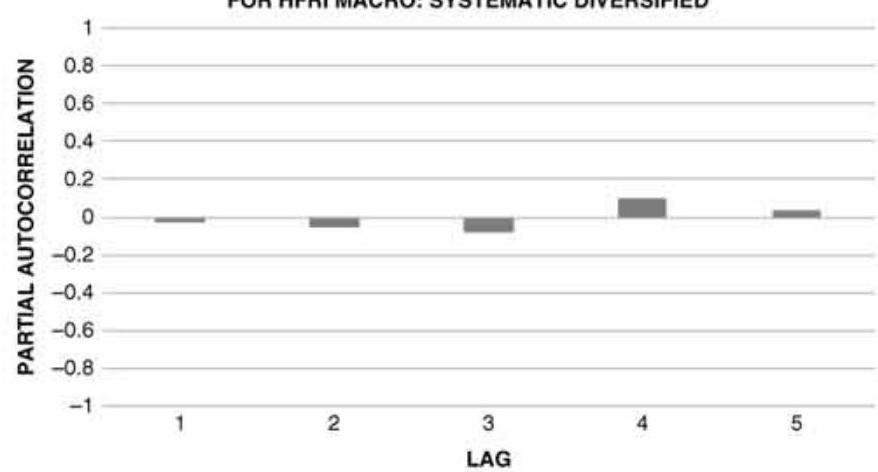
\includegraphics[max width=\textwidth]{2024_04_09_95e1381b1a9de89facc2g-4(1)}
\end{center}

PARTIAL AUTOCORRELATION FUNCTION FOR HFRI MACRO (TOTAL)

\begin{center}
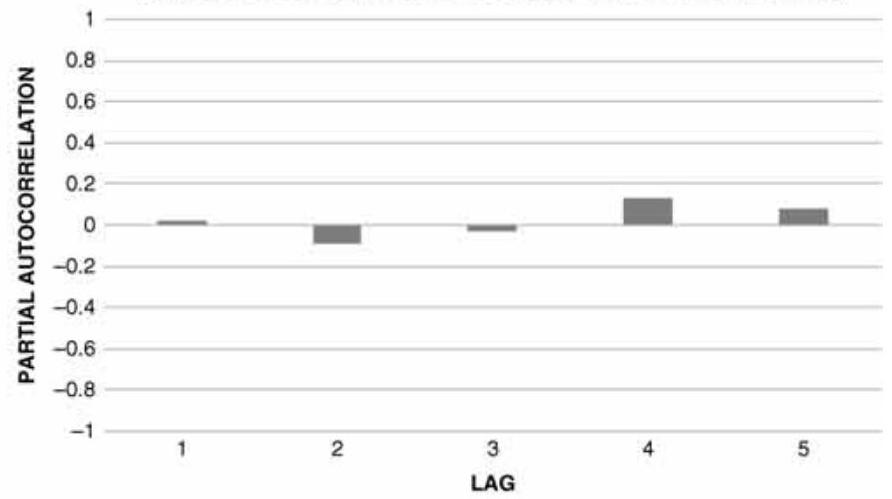
\includegraphics[max width=\textwidth]{2024_04_09_95e1381b1a9de89facc2g-4}
\end{center}

Histogram of HFRI Macro: Systematic Diversified Returns (Monthly) Jan. 2000-Dec. 2021

$$
\text { Bucket 2: }-6.2 \%<x<-5.2 \%
$$

$$
\begin{aligned}
& \text { Bucket 1: }- \text { Infinity } \%<x<-6.3 \\
& \text { Bucket 2: }-6.2 \%<x<-5.2 \% \\
& \text { Bucket 3: }-5.1 \%<x<-4.1 \% \\
& \text { Bucket 4: }-4.0 \%<x<-3.0 \% \\
& \text { Bucket 5: }-2.9 \%<x<-1.9 \% \\
& \text { Bucket 6: }-1.8 \%<x<-0.8 \% \\
& \text { Bucket 7: }-0.7 \%<x<1.4 \% \\
& \text { Bucket 8: } 1.5 \%<x<2.5 \% \\
& \text { Bucket } 9: 2.6 \%<x<3.6 \%
\end{aligned}
$$

Bucket 10: $3.7 \%<x<4.7 \%$

Bucket 11: $4.8 \%<x<5.9 \%$

Bucket 12: $6.0 \%<x<7.0 \%$

Bucket 13: $7.1 \%<x<$ Infinity \%

Histogram of HFRI Macro (Total) Returns (Monthly) Jan. 2000-Dec. 2021

120

\begin{center}
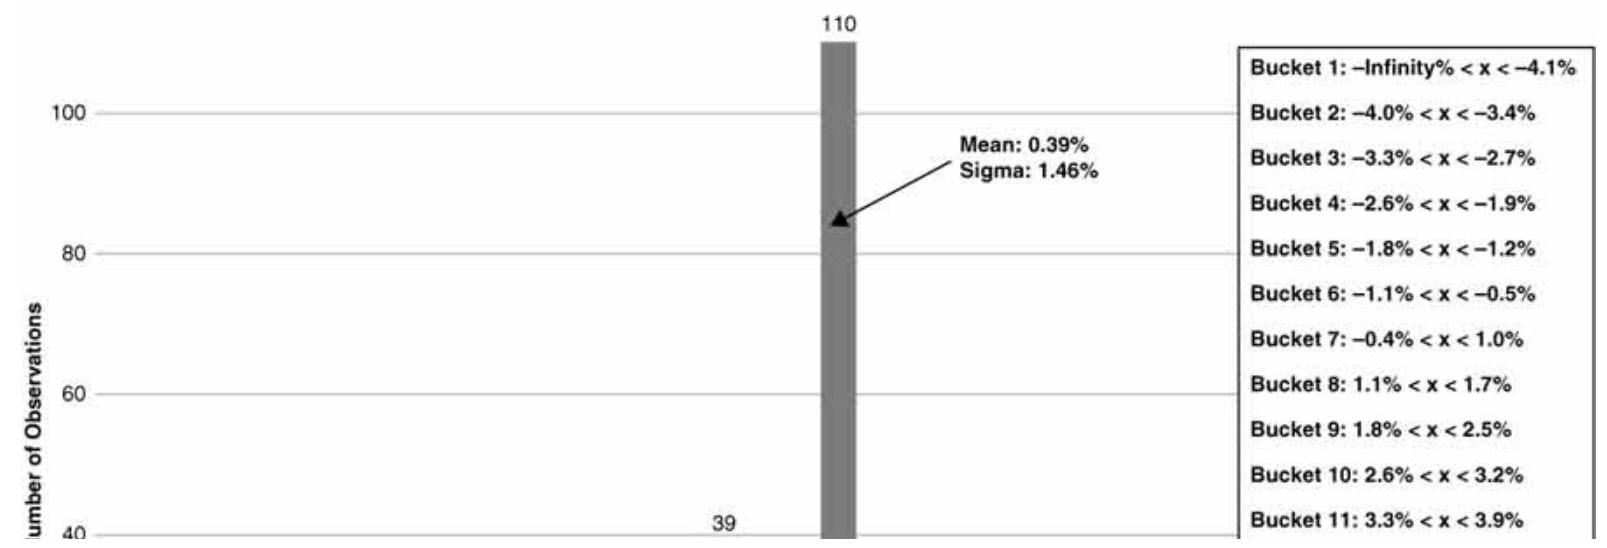
\includegraphics[max width=\textwidth]{2024_04_09_95e1381b1a9de89facc2g-4(2)}
\end{center}

HFRI Macro (Total) Return Buckets

\section*{Statistical Summary of Returns}
Key observations on the returns to systematic diversified funds that are consistent with economic reasoning are an essential component of knowledge and include the following:

\begin{enumerate}
  \item The historic return distribution of systematic diversified funds resembled that of a normal distribution, with no indication of a pronounced skew or fat tails (excess kurtosis).

  \item Volatility of returns was moderately low relative to world equities.

  \item Returns exhibited little or no autocorrelation.

  \item Maximum drawdown was much better than observed for global equities.

\end{enumerate}

Key observations on the returns to macro funds that are consistent with economic reasoning are an essential component of knowledge and include the following:

\begin{enumerate}
  \item The historic return distribution of Macro (Total) resembled that of a normal distribution, with no indication of a pronounced skew or fat tails (excess kurtosis).

  \item Volatility of returns was low relative to world equities.

  \item Returns exhibited little or no autocorrelation.

  \item Maximum drawdown was much better than observed for global equities.

\end{enumerate}

\end{document}